\documentclass[10pt]{article} % For LaTeX2e
\usepackage[preprint]{tmlr}

% If accepted, instead use the following line for the camera-ready submission:
%\usepackage[accepted]{tmlr}
% To de-anonymize and remove mentions to TMLR (for example for posting to preprint servers), instead use the following:
%\usepackage[preprint]{tmlr}

% Optional math commands from https://github.com/goodfeli/dlbook_notation.
%%%%% NEW MATH DEFINITIONS %%%%%

\usepackage{amsmath,amsfonts,bm}

% Mark sections of captions for referring to divisions of figures
\newcommand{\figleft}{{\em (Left)}}
\newcommand{\figcenter}{{\em (Center)}}
\newcommand{\figright}{{\em (Right)}}
\newcommand{\figtop}{{\em (Top)}}
\newcommand{\figbottom}{{\em (Bottom)}}
\newcommand{\captiona}{{\em (a)}}
\newcommand{\captionb}{{\em (b)}}
\newcommand{\captionc}{{\em (c)}}
\newcommand{\captiond}{{\em (d)}}

% Highlight a newly defined term
\newcommand{\newterm}[1]{{\bf #1}}


% Figure reference, lower-case.
\def\figref#1{figure~\ref{#1}}
% Figure reference, capital. For start of sentence
\def\Figref#1{Figure~\ref{#1}}
\def\twofigref#1#2{figures \ref{#1} and \ref{#2}}
\def\quadfigref#1#2#3#4{figures \ref{#1}, \ref{#2}, \ref{#3} and \ref{#4}}
% Section reference, lower-case.
\def\secref#1{section~\ref{#1}}
% Section reference, capital.
\def\Secref#1{Section~\ref{#1}}
% Reference to two sections.
\def\twosecrefs#1#2{sections \ref{#1} and \ref{#2}}
% Reference to three sections.
\def\secrefs#1#2#3{sections \ref{#1}, \ref{#2} and \ref{#3}}
% Reference to an equation, lower-case.
\def\eqref#1{equation~\ref{#1}}
% Reference to an equation, upper case
\def\Eqref#1{Equation~\ref{#1}}
% A raw reference to an equation---avoid using if possible
\def\plaineqref#1{\ref{#1}}
% Reference to a chapter, lower-case.
\def\chapref#1{chapter~\ref{#1}}
% Reference to an equation, upper case.
\def\Chapref#1{Chapter~\ref{#1}}
% Reference to a range of chapters
\def\rangechapref#1#2{chapters\ref{#1}--\ref{#2}}
% Reference to an algorithm, lower-case.
\def\algref#1{algorithm~\ref{#1}}
% Reference to an algorithm, upper case.
\def\Algref#1{Algorithm~\ref{#1}}
\def\twoalgref#1#2{algorithms \ref{#1} and \ref{#2}}
\def\Twoalgref#1#2{Algorithms \ref{#1} and \ref{#2}}
% Reference to a part, lower case
\def\partref#1{part~\ref{#1}}
% Reference to a part, upper case
\def\Partref#1{Part~\ref{#1}}
\def\twopartref#1#2{parts \ref{#1} and \ref{#2}}

\def\ceil#1{\lceil #1 \rceil}
\def\floor#1{\lfloor #1 \rfloor}
\def\1{\bm{1}}
\newcommand{\train}{\mathcal{D}}
\newcommand{\valid}{\mathcal{D_{\mathrm{valid}}}}
\newcommand{\test}{\mathcal{D_{\mathrm{test}}}}

\def\eps{{\epsilon}}


% Random variables
\def\reta{{\textnormal{$\eta$}}}
\def\ra{{\textnormal{a}}}
\def\rb{{\textnormal{b}}}
\def\rc{{\textnormal{c}}}
\def\rd{{\textnormal{d}}}
\def\re{{\textnormal{e}}}
\def\rf{{\textnormal{f}}}
\def\rg{{\textnormal{g}}}
\def\rh{{\textnormal{h}}}
\def\ri{{\textnormal{i}}}
\def\rj{{\textnormal{j}}}
\def\rk{{\textnormal{k}}}
\def\rl{{\textnormal{l}}}
% rm is already a command, just don't name any random variables m
\def\rn{{\textnormal{n}}}
\def\ro{{\textnormal{o}}}
\def\rp{{\textnormal{p}}}
\def\rq{{\textnormal{q}}}
\def\rr{{\textnormal{r}}}
\def\rs{{\textnormal{s}}}
\def\rt{{\textnormal{t}}}
\def\ru{{\textnormal{u}}}
\def\rv{{\textnormal{v}}}
\def\rw{{\textnormal{w}}}
\def\rx{{\textnormal{x}}}
\def\ry{{\textnormal{y}}}
\def\rz{{\textnormal{z}}}

% Random vectors
\def\rvepsilon{{\mathbf{\epsilon}}}
\def\rvtheta{{\mathbf{\theta}}}
\def\rva{{\mathbf{a}}}
\def\rvb{{\mathbf{b}}}
\def\rvc{{\mathbf{c}}}
\def\rvd{{\mathbf{d}}}
\def\rve{{\mathbf{e}}}
\def\rvf{{\mathbf{f}}}
\def\rvg{{\mathbf{g}}}
\def\rvh{{\mathbf{h}}}
\def\rvu{{\mathbf{i}}}
\def\rvj{{\mathbf{j}}}
\def\rvk{{\mathbf{k}}}
\def\rvl{{\mathbf{l}}}
\def\rvm{{\mathbf{m}}}
\def\rvn{{\mathbf{n}}}
\def\rvo{{\mathbf{o}}}
\def\rvp{{\mathbf{p}}}
\def\rvq{{\mathbf{q}}}
\def\rvr{{\mathbf{r}}}
\def\rvs{{\mathbf{s}}}
\def\rvt{{\mathbf{t}}}
\def\rvu{{\mathbf{u}}}
\def\rvv{{\mathbf{v}}}
\def\rvw{{\mathbf{w}}}
\def\rvx{{\mathbf{x}}}
\def\rvy{{\mathbf{y}}}
\def\rvz{{\mathbf{z}}}

% Elements of random vectors
\def\erva{{\textnormal{a}}}
\def\ervb{{\textnormal{b}}}
\def\ervc{{\textnormal{c}}}
\def\ervd{{\textnormal{d}}}
\def\erve{{\textnormal{e}}}
\def\ervf{{\textnormal{f}}}
\def\ervg{{\textnormal{g}}}
\def\ervh{{\textnormal{h}}}
\def\ervi{{\textnormal{i}}}
\def\ervj{{\textnormal{j}}}
\def\ervk{{\textnormal{k}}}
\def\ervl{{\textnormal{l}}}
\def\ervm{{\textnormal{m}}}
\def\ervn{{\textnormal{n}}}
\def\ervo{{\textnormal{o}}}
\def\ervp{{\textnormal{p}}}
\def\ervq{{\textnormal{q}}}
\def\ervr{{\textnormal{r}}}
\def\ervs{{\textnormal{s}}}
\def\ervt{{\textnormal{t}}}
\def\ervu{{\textnormal{u}}}
\def\ervv{{\textnormal{v}}}
\def\ervw{{\textnormal{w}}}
\def\ervx{{\textnormal{x}}}
\def\ervy{{\textnormal{y}}}
\def\ervz{{\textnormal{z}}}

% Random matrices
\def\rmA{{\mathbf{A}}}
\def\rmB{{\mathbf{B}}}
\def\rmC{{\mathbf{C}}}
\def\rmD{{\mathbf{D}}}
\def\rmE{{\mathbf{E}}}
\def\rmF{{\mathbf{F}}}
\def\rmG{{\mathbf{G}}}
\def\rmH{{\mathbf{H}}}
\def\rmI{{\mathbf{I}}}
\def\rmJ{{\mathbf{J}}}
\def\rmK{{\mathbf{K}}}
\def\rmL{{\mathbf{L}}}
\def\rmM{{\mathbf{M}}}
\def\rmN{{\mathbf{N}}}
\def\rmO{{\mathbf{O}}}
\def\rmP{{\mathbf{P}}}
\def\rmQ{{\mathbf{Q}}}
\def\rmR{{\mathbf{R}}}
\def\rmS{{\mathbf{S}}}
\def\rmT{{\mathbf{T}}}
\def\rmU{{\mathbf{U}}}
\def\rmV{{\mathbf{V}}}
\def\rmW{{\mathbf{W}}}
\def\rmX{{\mathbf{X}}}
\def\rmY{{\mathbf{Y}}}
\def\rmZ{{\mathbf{Z}}}

% Elements of random matrices
\def\ermA{{\textnormal{A}}}
\def\ermB{{\textnormal{B}}}
\def\ermC{{\textnormal{C}}}
\def\ermD{{\textnormal{D}}}
\def\ermE{{\textnormal{E}}}
\def\ermF{{\textnormal{F}}}
\def\ermG{{\textnormal{G}}}
\def\ermH{{\textnormal{H}}}
\def\ermI{{\textnormal{I}}}
\def\ermJ{{\textnormal{J}}}
\def\ermK{{\textnormal{K}}}
\def\ermL{{\textnormal{L}}}
\def\ermM{{\textnormal{M}}}
\def\ermN{{\textnormal{N}}}
\def\ermO{{\textnormal{O}}}
\def\ermP{{\textnormal{P}}}
\def\ermQ{{\textnormal{Q}}}
\def\ermR{{\textnormal{R}}}
\def\ermS{{\textnormal{S}}}
\def\ermT{{\textnormal{T}}}
\def\ermU{{\textnormal{U}}}
\def\ermV{{\textnormal{V}}}
\def\ermW{{\textnormal{W}}}
\def\ermX{{\textnormal{X}}}
\def\ermY{{\textnormal{Y}}}
\def\ermZ{{\textnormal{Z}}}

% Vectors
\def\vzero{{\bm{0}}}
\def\vone{{\bm{1}}}
\def\vmu{{\bm{\mu}}}
\def\vtheta{{\bm{\theta}}}
\def\va{{\bm{a}}}
\def\vb{{\bm{b}}}
\def\vc{{\bm{c}}}
\def\vd{{\bm{d}}}
\def\ve{{\bm{e}}}
\def\vf{{\bm{f}}}
\def\vg{{\bm{g}}}
\def\vh{{\bm{h}}}
\def\vi{{\bm{i}}}
\def\vj{{\bm{j}}}
\def\vk{{\bm{k}}}
\def\vl{{\bm{l}}}
\def\vm{{\bm{m}}}
\def\vn{{\bm{n}}}
\def\vo{{\bm{o}}}
\def\vp{{\bm{p}}}
\def\vq{{\bm{q}}}
\def\vr{{\bm{r}}}
\def\vs{{\bm{s}}}
\def\vt{{\bm{t}}}
\def\vu{{\bm{u}}}
\def\vv{{\bm{v}}}
\def\vw{{\bm{w}}}
\def\vx{{\bm{x}}}
\def\vy{{\bm{y}}}
\def\vz{{\bm{z}}}

% Elements of vectors
\def\evalpha{{\alpha}}
\def\evbeta{{\beta}}
\def\evepsilon{{\epsilon}}
\def\evlambda{{\lambda}}
\def\evomega{{\omega}}
\def\evmu{{\mu}}
\def\evpsi{{\psi}}
\def\evsigma{{\sigma}}
\def\evtheta{{\theta}}
\def\eva{{a}}
\def\evb{{b}}
\def\evc{{c}}
\def\evd{{d}}
\def\eve{{e}}
\def\evf{{f}}
\def\evg{{g}}
\def\evh{{h}}
\def\evi{{i}}
\def\evj{{j}}
\def\evk{{k}}
\def\evl{{l}}
\def\evm{{m}}
\def\evn{{n}}
\def\evo{{o}}
\def\evp{{p}}
\def\evq{{q}}
\def\evr{{r}}
\def\evs{{s}}
\def\evt{{t}}
\def\evu{{u}}
\def\evv{{v}}
\def\evw{{w}}
\def\evx{{x}}
\def\evy{{y}}
\def\evz{{z}}

% Matrix
\def\mA{{\bm{A}}}
\def\mB{{\bm{B}}}
\def\mC{{\bm{C}}}
\def\mD{{\bm{D}}}
\def\mE{{\bm{E}}}
\def\mF{{\bm{F}}}
\def\mG{{\bm{G}}}
\def\mH{{\bm{H}}}
\def\mI{{\bm{I}}}
\def\mJ{{\bm{J}}}
\def\mK{{\bm{K}}}
\def\mL{{\bm{L}}}
\def\mM{{\bm{M}}}
\def\mN{{\bm{N}}}
\def\mO{{\bm{O}}}
\def\mP{{\bm{P}}}
\def\mQ{{\bm{Q}}}
\def\mR{{\bm{R}}}
\def\mS{{\bm{S}}}
\def\mT{{\bm{T}}}
\def\mU{{\bm{U}}}
\def\mV{{\bm{V}}}
\def\mW{{\bm{W}}}
\def\mX{{\bm{X}}}
\def\mY{{\bm{Y}}}
\def\mZ{{\bm{Z}}}
\def\mBeta{{\bm{\beta}}}
\def\mPhi{{\bm{\Phi}}}
\def\mLambda{{\bm{\Lambda}}}
\def\mSigma{{\bm{\Sigma}}}

% Tensor
\DeclareMathAlphabet{\mathsfit}{\encodingdefault}{\sfdefault}{m}{sl}
\SetMathAlphabet{\mathsfit}{bold}{\encodingdefault}{\sfdefault}{bx}{n}
\newcommand{\tens}[1]{\bm{\mathsfit{#1}}}
\def\tA{{\tens{A}}}
\def\tB{{\tens{B}}}
\def\tC{{\tens{C}}}
\def\tD{{\tens{D}}}
\def\tE{{\tens{E}}}
\def\tF{{\tens{F}}}
\def\tG{{\tens{G}}}
\def\tH{{\tens{H}}}
\def\tI{{\tens{I}}}
\def\tJ{{\tens{J}}}
\def\tK{{\tens{K}}}
\def\tL{{\tens{L}}}
\def\tM{{\tens{M}}}
\def\tN{{\tens{N}}}
\def\tO{{\tens{O}}}
\def\tP{{\tens{P}}}
\def\tQ{{\tens{Q}}}
\def\tR{{\tens{R}}}
\def\tS{{\tens{S}}}
\def\tT{{\tens{T}}}
\def\tU{{\tens{U}}}
\def\tV{{\tens{V}}}
\def\tW{{\tens{W}}}
\def\tX{{\tens{X}}}
\def\tY{{\tens{Y}}}
\def\tZ{{\tens{Z}}}


% Graph
\def\gA{{\mathcal{A}}}
\def\gB{{\mathcal{B}}}
\def\gC{{\mathcal{C}}}
\def\gD{{\mathcal{D}}}
\def\gE{{\mathcal{E}}}
\def\gF{{\mathcal{F}}}
\def\gG{{\mathcal{G}}}
\def\gH{{\mathcal{H}}}
\def\gI{{\mathcal{I}}}
\def\gJ{{\mathcal{J}}}
\def\gK{{\mathcal{K}}}
\def\gL{{\mathcal{L}}}
\def\gM{{\mathcal{M}}}
\def\gN{{\mathcal{N}}}
\def\gO{{\mathcal{O}}}
\def\gP{{\mathcal{P}}}
\def\gQ{{\mathcal{Q}}}
\def\gR{{\mathcal{R}}}
\def\gS{{\mathcal{S}}}
\def\gT{{\mathcal{T}}}
\def\gU{{\mathcal{U}}}
\def\gV{{\mathcal{V}}}
\def\gW{{\mathcal{W}}}
\def\gX{{\mathcal{X}}}
\def\gY{{\mathcal{Y}}}
\def\gZ{{\mathcal{Z}}}

% Sets
\def\sA{{\mathbb{A}}}
\def\sB{{\mathbb{B}}}
\def\sC{{\mathbb{C}}}
\def\sD{{\mathbb{D}}}
% Don't use a set called E, because this would be the same as our symbol
% for expectation.
\def\sF{{\mathbb{F}}}
\def\sG{{\mathbb{G}}}
\def\sH{{\mathbb{H}}}
\def\sI{{\mathbb{I}}}
\def\sJ{{\mathbb{J}}}
\def\sK{{\mathbb{K}}}
\def\sL{{\mathbb{L}}}
\def\sM{{\mathbb{M}}}
\def\sN{{\mathbb{N}}}
\def\sO{{\mathbb{O}}}
\def\sP{{\mathbb{P}}}
\def\sQ{{\mathbb{Q}}}
\def\sR{{\mathbb{R}}}
\def\sS{{\mathbb{S}}}
\def\sT{{\mathbb{T}}}
\def\sU{{\mathbb{U}}}
\def\sV{{\mathbb{V}}}
\def\sW{{\mathbb{W}}}
\def\sX{{\mathbb{X}}}
\def\sY{{\mathbb{Y}}}
\def\sZ{{\mathbb{Z}}}

% Entries of a matrix
\def\emLambda{{\Lambda}}
\def\emA{{A}}
\def\emB{{B}}
\def\emC{{C}}
\def\emD{{D}}
\def\emE{{E}}
\def\emF{{F}}
\def\emG{{G}}
\def\emH{{H}}
\def\emI{{I}}
\def\emJ{{J}}
\def\emK{{K}}
\def\emL{{L}}
\def\emM{{M}}
\def\emN{{N}}
\def\emO{{O}}
\def\emP{{P}}
\def\emQ{{Q}}
\def\emR{{R}}
\def\emS{{S}}
\def\emT{{T}}
\def\emU{{U}}
\def\emV{{V}}
\def\emW{{W}}
\def\emX{{X}}
\def\emY{{Y}}
\def\emZ{{Z}}
\def\emSigma{{\Sigma}}

% entries of a tensor
% Same font as tensor, without \bm wrapper
\newcommand{\etens}[1]{\mathsfit{#1}}
\def\etLambda{{\etens{\Lambda}}}
\def\etA{{\etens{A}}}
\def\etB{{\etens{B}}}
\def\etC{{\etens{C}}}
\def\etD{{\etens{D}}}
\def\etE{{\etens{E}}}
\def\etF{{\etens{F}}}
\def\etG{{\etens{G}}}
\def\etH{{\etens{H}}}
\def\etI{{\etens{I}}}
\def\etJ{{\etens{J}}}
\def\etK{{\etens{K}}}
\def\etL{{\etens{L}}}
\def\etM{{\etens{M}}}
\def\etN{{\etens{N}}}
\def\etO{{\etens{O}}}
\def\etP{{\etens{P}}}
\def\etQ{{\etens{Q}}}
\def\etR{{\etens{R}}}
\def\etS{{\etens{S}}}
\def\etT{{\etens{T}}}
\def\etU{{\etens{U}}}
\def\etV{{\etens{V}}}
\def\etW{{\etens{W}}}
\def\etX{{\etens{X}}}
\def\etY{{\etens{Y}}}
\def\etZ{{\etens{Z}}}

% The true underlying data generating distribution
\newcommand{\pdata}{p_{\rm{data}}}
% The empirical distribution defined by the training set
\newcommand{\ptrain}{\hat{p}_{\rm{data}}}
\newcommand{\Ptrain}{\hat{P}_{\rm{data}}}
% The model distribution
\newcommand{\pmodel}{p_{\rm{model}}}
\newcommand{\Pmodel}{P_{\rm{model}}}
\newcommand{\ptildemodel}{\tilde{p}_{\rm{model}}}
% Stochastic autoencoder distributions
\newcommand{\pencode}{p_{\rm{encoder}}}
\newcommand{\pdecode}{p_{\rm{decoder}}}
\newcommand{\precons}{p_{\rm{reconstruct}}}

\newcommand{\laplace}{\mathrm{Laplace}} % Laplace distribution

\newcommand{\E}{\mathbb{E}}
\newcommand{\Ls}{\mathcal{L}}
\newcommand{\R}{\mathbb{R}}
\newcommand{\emp}{\tilde{p}}
\newcommand{\lr}{\alpha}
\newcommand{\reg}{\lambda}
\newcommand{\rect}{\mathrm{rectifier}}
\newcommand{\softmax}{\mathrm{softmax}}
\newcommand{\sigmoid}{\sigma}
\newcommand{\softplus}{\zeta}
\newcommand{\KL}{D_{\mathrm{KL}}}
\newcommand{\Var}{\mathrm{Var}}
\newcommand{\standarderror}{\mathrm{SE}}
\newcommand{\Cov}{\mathrm{Cov}}
% Wolfram Mathworld says $L^2$ is for function spaces and $\ell^2$ is for vectors
% But then they seem to use $L^2$ for vectors throughout the site, and so does
% wikipedia.
\newcommand{\normlzero}{L^0}
\newcommand{\normlone}{L^1}
\newcommand{\normltwo}{L^2}
\newcommand{\normlp}{L^p}
\newcommand{\normmax}{L^\infty}

\newcommand{\parents}{Pa} % See usage in notation.tex. Chosen to match Daphne's book.

\DeclareMathOperator*{\argmax}{arg\,max}
\DeclareMathOperator*{\argmin}{arg\,min}

\DeclareMathOperator{\sign}{sign}
\DeclareMathOperator{\Tr}{Tr}
\let\ab\allowbreak


\usepackage{graphicx}
\usepackage{hyperref}
\usepackage{url}


\title{Walrus Co. \\
Introduction to Data Science 2023 \\
Technical Report}

% Authors must not appear in the submitted version. They should be hidden
% as long as the tmlr package is used without the [accepted] or [preprint] options.
% Non-anonymous submissions will be rejected without review.

\author{\name Christian Cardin
      \AND
      \name Elva Granados Escartin
      \AND
      \name Julia Pukarinen}

% The \author macro works with any number of authors. Use \AND 
% to separate the names and addresses of multiple authors.

\newcommand{\fix}{\marginpar{FIX}}
\newcommand{\new}{\marginpar{NEW}}

\def\month{MM}  % Insert correct month for camera-ready version
\def\year{YYYY} % Insert correct year for camera-ready version
\def\openreview{\url{https://openreview.net/forum?id=XXXX}} % Insert correct link to OpenReview for camera-ready version


\begin{document}


\maketitle

\begin{abstract}
In this technical report, we introduce the technicalities of our project for the course Introduction to Data Science 2023, and enter the details on few selected highlights.
\end{abstract}

\section{Motivation}

Our motivation for the project was to understand the situation of the economic cycle, based on US historical economic data, and give traders an insight of possible opportunities. Our purpose was to predict short-term performance of financial indices based on macroeconomic data and other market sector indices. We also wanted to learn the correlation between market indices and macroeconomic data.

\section{Running the Code}
We recommand having a version of Python 3.8 or superior, and an updated version of pip. Our project is hosted on GitHub at the address \href{https://github.com/sechlol/intro_ds_2023}{https://github.com/sechlol/intro\_ds\_2023}. First of all, clone the repository. Then, locate the file \texttt{requirements.txt} in the project root folder and install the required packages with the command \texttt{pip install -r requirements.txt}. To run the code, simply call \texttt{python main.py}.

\section{Software Architecture}

\begin{figure}[h]
  \begin{center}
    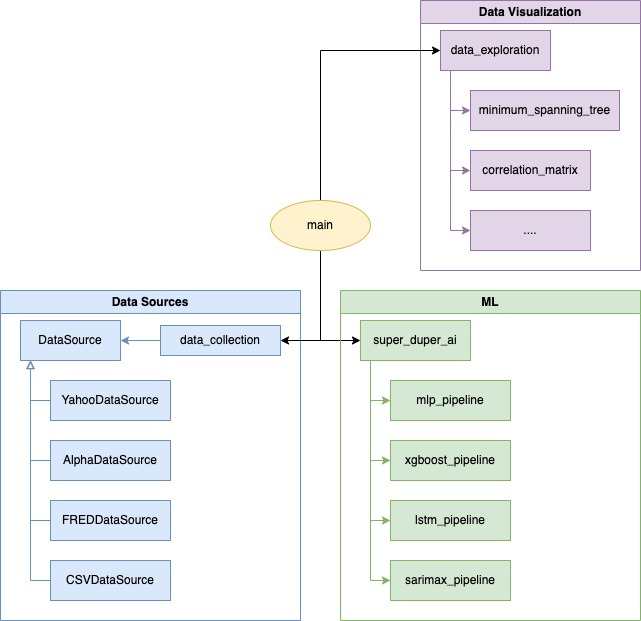
\includegraphics[width=0.6\textwidth]{img/arch.jpg}
  \end{center}
  \caption{Simple view on project architecture}
  \label{fig:arch}
  \end{figure}

The project is structured into distinct modules, each with a specific role, reflecting the best practices of clear programming. Breaking down the code into these separate units encourages modularity and encapsulation, which, in turn, enhances code clarity and makes it more understandable. This organized approach not only benefits human readability but also simplifies maintenance and troubleshooting, as modifications are confined to their respective modules, reducing unexpected side effects.

At the core of the codebase, the \texttt{main.py} file serves as the project's entry point, orchestrating the execution by sequentially calling these individual modules. This method promotes a clean and logical structure, enabling developers to navigate the codebase more easily.

\begin{enumerate}
  \item Data Collection: Each data source is queried independently, resulting in an array of time-series dataframes. Each dataframe contains different finance data features, which is then combined together in a unique large dataframe. See Section~\ref{sec:data} for more information on data collection.
  \item Machine Learning: The dataset is passed to the \texttt{super\_duper\_ai.py} script, which contains multiple pipelines for the training and evaluation of machine learning and deep learning models. The module performs some independent manipulations on the dataset, like normalization and augmentation.
  \item Data Visualization: From the original dataset, this module is responsible for extracting interesting insights from the data and create plots to be then analyzed.
\end{enumerate}

A simple schematic view on the project software architecture is depicted in Fig.~\ref{fig:arch}

\section{Data Collection}\label{sec:data}

\subsection{DataSources}
There is a great variety of services that offer high quality economic data API; however, the almost totality of them ask for a premium price to access their data. We identified a handful of services that, previous registration, allowed users to access their data free of charge, with limitations imposed by usage volume of their APIs.
For the daily price action of the major market indices, we chose \textbf{Yahoo! Finance}\footnote{\href{https://finance.yahoo.com/}{https://finance.yahoo.com/}}, for which a convenient python library (\texttt{yfinance}\footnote{\href{https://pypi.org/project/yfinance/}{https://pypi.org/project/yfinance/}}) is available to easily retrieve timeseries for stocks data given their unique identifier (ticker). From Yahoo finance we got the data on S\&P 500 and the 11 industry sectors: Information Technology, Health Care, Financials, Consumer Discretionary, Communication Services, Industrials, Consumer Staples, Energy, Utilities, Real Estate, and Materials. 

For macroeconomic data, we resorted to \textbf{FRED}\footnote{\href{https://fred.stlouisfed.org/}{https://fred.stlouisfed.org/}} (Federal Reserve Economic Data), which contains a treasure of data from the United States dating back as early as the beginning of the $20^{th}$ century.

For special technical indicators, we identified \textbf{AlphaVantage}\footnote{\href{https://www.alphavantage.co/documentation/}{https://www.alphavantage.co/documentation/}} as a valid source. Unfortunately, we encountered some troubles with the latter: their free tier strongly limits the frequency of queries that a user can make, so we had to keep the number of data features retrieved from this source quite low.

%Indices:
%Real Gross Domestic Product, Unemployment rate, Industrial Production: Total Index, 10-Year Treasury Constant Maturity Minus 2-Year Treasury Constant Maturity, 10-Year Treasury Constant Maturity Minus 3-Month Treasury Constant Maturity, All Employees Total Nonfarm, Initial Jobless Claims, Consumer Sentiment University of Michigan, Manufacturers' New Orders: Durable Goods, Federal Funds Effective Rate, CBOE Volatility Index: VIX, Crude Oil Prices: West Texas Intermediate (WTI) - Cushing Oklahoma, Consumer Price Index for All Urban Consumers: All Items in U.S. City Average, Producer Price Index by Commodity: All Commodities, Average Weekly Hours of Production and Nonsupervisory Employees Manufacturing, Manufacturers' New Orders: Nondefense Capital Goods Excluding Aircraft, Manufacturers' New Orders: Consumer Goods and All Employees Truck Transportation.

\section{Preprocessing}

The data of the indices are presented as a function of time. The sampling frequency varies between indices. In particular, stock data come with a Business daily frequency (5 times per week), and macroeconomic data is usually released at monthly or quarterly cadence. We had to decide whether to collapse the daily data to monthly or expand the monthly data to daily in order to match the data collected at the two different sampling frequencies. We decided to expand the monthly data to daily by giving each day of the month the same value (forward filling). 
To keep a consistent dataset, we decided to drop each row with missing data, meaning that we trimmed the dataset to the earliest time for which we had complete data, until today. Unfortunately for us, the timespan of each economic feature varied greatly. Some features like GDP (Gross Domestic Product) were available starting from the early 1900, but some indices like Real Estate (XLRE) and Communication services (XLC) were only available starting from 2018, which would limit our historical timespan too much. We then decided to drop the last two indices, allowing us to collect data starting from 1998 onward.

\section{Learning Tasks}
To answer one of our research question "Why aren't ML experts all billionaires, already?" we tried to predict whether the stock market would be profitable in the near future. This resuted in a binary prediction problem: predict a 1 if the ticker of interest after X periods will be greater than today's price, else predict a 0 if the price will be lower. Both ticker and number of periods are variables that can be tuned at will. We focused mainly on the S\&P 500 index (\textbf{SPY}), and tried a multitude of periods, ranging from 1 day to 2 months.

We implemented three algorithms, here we only discuss the hyperparameter tuning, while more general details on the algorithm and the results are highlighted in the blog.

\begin{description}
  \item[\textbf{XGBoost}:] using the dedicated python library.\footnote{\href{https://github.com/dmlc/xgboost}{https://github.com/dmlc/xgboost}} In our specific implementation, we set several hyperparameters for XGBoost to optimize its performance. We use "binary:logistic" as the prediction objective, which means the model will output the probability of a positive return, ranging from 0 to 1. To evaluate the quality of predictions, we employ metrics such as "error" for binary classification error, "auc" for the Area under the curve, and "logloss" for the negative log likelihood. For training and model evaluation, we use a 5-fold cross-validation approach. The trees in XGBoost use the "hist" algorithm, which is a faster histogram-optimized approximate greedy algorithm, with specific settings such as "max\_depth=3" and "min\_child\_weight=4." Early stopping is also implemented if there are no improvements in 20 rounds.
  
  \item[\textbf{Multilayer Perceptron}:] from Sci-Kit package.\footnote{\href{https://scikit-learn.org/stable/index.html}{https://scikit-learn.org/stable/index.html}} We employ a neural network architecture with 100 hidden layers. This deep architecture allows the model to learn intricate and hierarchical patterns from the data. The optimizer used is Stochastic Gradient Descent (SGD) with a constant learning rate. The batch size for training is set to 64, which determines how many data points are used in each iteration to update the model. Early stopping is a mechanism implemented to prevent overfitting and save computational resources. If there are no improvements in the model's performance for 20 consecutive iterations, the training process is terminated.
  
  \item [\textbf{LSTM / GRU}:] "Long-Short term memory" and "Gated Recurrent Unit", from Keras.\footnote{\href{https://keras.io/}{https://keras.io/}} In our experimentation, we explored various model architectures based on both LSTM and GRU networks. These models consisted of 50 layers with a hyperbolic tangent (tanh) activation function. The tanh activation function introduces non-linearity into the network, allowing it to capture complex patterns. The models included a unit normalization layer, which can enhance the training stability and convergence of the network. Each architecture culminated with a 3-layer dense classifier, providing the final prediction output. The optimizer utilized in this setup is Stochastic Gradient Descent (SGD) with a learning rate of 0.01. For loss computation, Binary Cross-Entropy is chosen as the loss function. This is a common choice for binary classification tasks, where the model evaluates how well its predictions match the actual outcomes. Binary Accuracy is used as the evaluation metric, assessing the model's ability to predict binary classifications accurately.

\end{description}
More information on these algorithms are found in the blog.

\subsection{Challenges}
Developing good ML algorithms is hard. It's easy to blindly train a model, and be fooled by the good performance in the training data. The biggest challenge for us was to find a good set of hyperparamters for our models to improve its inference accuracy on unseen test data. Ultimately, we were not able to reach any meaningful prediction that was better than random guess. This made us think that we should have spent more time experimenting with the features we included in our training dataset, rather then focusing on hyperparmeter tuning. 


\section{Exploratory Data Analysis}

Correlation is a statistical measure that describes how two assets are related. It can give perspective on the overall nature of the market. We use rolling Pearson correlation with pandas. The window used for the rolling correlation was one month or one year. It depended on whether we were dealing with an index for which daily or monthly data was available. A monthly correlation could be calculated for the indices for which daily data was obtained. Although the monthly data was extended to daily, no monthly correlation could be calculated for those indices, because the value remained the same throughout the month. Thus, one year had to be selected as a window whenever there was an index with monthly data.

The scale varies between -1 and +1. Correlation of -1 indicates a perfectly linear negative correlation and +1 indicates a perfectly linear positive correlation. Correlation of 0 indicates that there is no linear dependency between the two assets. So the higher the positive correlation, the more strongly the two assets vary together, and the higher the negative correlation, the more strongly they vary together but in opposite directions.

\section{Visualizations}

We wanted to visualize indicators and market indices to look at their performances and correlations as well as the performance of the machine learning algorithms used.

We plotted basic plots of the performance of indices and markets in time, picking different combinations, depending on what features were being analyzed. On these basic plots the times of financial crises were highlighted in grey to add to the readability.

To show correlations we used correlation matrices and rolling correlations.
We used Plotly's interactive Slider feature to help us show the rolling correlation as a function of time between two indices. We also used Plotly's interactive minimum spanning tree to show how all indices behave in relation to each other within a given time interval. Using the minimum spanning tree, we obtained information about which indices show the strongest and weakest correlations with each other, annualised returns and annualised volatility.

To assess the performance of the ML algorithms we plotted accuracy metrics and confusion matrices. 


\section{Communication of Results}

The results obtained from the analysis and predictions are reported in a blog post, available at the GitHub-hosted address \href{https://sechlol.github.io/intro\_ds\_2023/}{https://sechlol.github.io/intro\_ds\_2023/}. The HTML pages are generated with Quarto\footnote{\href{https://quarto.org/}{https://quarto.org/}}, an open source scientific publishing system that automatically generates HTML pages from a markdown file, or Jupyter notebook.

In this text we communicate the results from the machine learning algorithms as well as some more general economic analysis of our data. For the sake of knowledge and speculation.

In the part where the results of the machine learning algorithms are considered, we explain the algorithms used and go through the results, comparing them together using accuracy metrics. 

\section{Final Considerations}

Unfortunately, the outcome was not as desired. Our predictions were as good as a random guess, and we won't be getting our Lambos and Range Rovers any time soon. 

So our end result cannot be said to be actionable, despite our best efforts. This was expected, because it is not so easy to predict the stock market, even taking into consideration a wide array of macroeconomic indicators. Indeed, if it was so easy everyone would do it, and in the blink of an eye, the efficiency of the markets would take care of terminating the party before things get out of hand. Nevertheless we wanted to try, because it seemed like an interesting learning opportunity, plus you never know...

Nevertheless, we managed to build a good framework for data collection, processing and analysis that can be used for further development, for example in the case of getting access to more data, or adding new ML models. For us all, it was an exemplary learning experience encompassing all steps in the life cycle of a data science project, from finding the data to presenting the end results.

It is worth mentioning that one component of our group was dealing with many of these topics for the first time, and gained an important amount of insights, from the details of using Git for collaborative coding to the core ideas in data science and even getting an excuse to study a little economic theory. So it was a great opportunity with a splendid learning outcome.

Another component of our group didn't know much about the subject before the project. They would definitely have gotten more out of the work and been able to make a wider contribution if they had understood the subject more. Git as an environment was completely new and learning its basics was very useful. Using classes with Python was new and interesting. It was also nice to recall some methods of data collection. Learning how to make interactive graphs was pleasant and it certainly will give great opportunities for presenting some results in the future.

Future opportunities may lie in focusing the analysis in more specific, and less watched areas of the markets, for finding lurking market inefficiencies, i. e. potential profits.

\end{document}
